\documentclass[12pt,english,titlepage,a4paper]{article}

\usepackage{babel}
\usepackage{natbib}
\usepackage{graphicx}
\usepackage{tabularx}
\usepackage{float}
\usepackage{hyperref}

\hypersetup{
    colorlinks=true,
    linkcolor=black,
    filecolor=magenta,      
    urlcolor=blue,
    citecolor=blue
}

\begin{document}
%===========================================================
\begin{titlepage}
\begin{center}

\textbf{\LARGE How Victims Describe Cybercrime Incidents: A Text Analysis Approach}

\bigskip\bigskip
\textbf{Bachelor Thesis}

\bigskip
\textbf{Mundher A. Y. Al-Ahmadi}



\vfill
Chair of Digital Innovation and Entrepreneurship\\ 
Faculty of Mathematics and Natural Sciences \\ 
Heinrich Heine University D\"usseldorf

\bigskip
\today

\bigskip
Supervisor: Prof. Dr. Steffi Haag \\
Second supervisor: Prof.\ Dr.\ Melanie Schmidt

\end{center}
\end{titlepage}

\thispagestyle{empty}\mbox{}\pagebreak
\setcounter{page}{0}




%===========================================================
% Table of Contents
%===========================================================

\tableofcontents
\pagebreak

%===========================================================
% Abstract
%===========================================================
\section*{Abstract}
\addcontentsline{toc}{section}{Abstract}
Cybercrime is a growing threat to both organizations and individuals. The financial damages caused by cybercrime are very high, but an under researched consequence of cybercrime is the psychological impact it has on victims.~\cite{horesearch} This paper aims to apply modern text analysis methods, namely topic modeling and sentiment analysis, to a corpus of stories of victims who have had encounters with cybercrime. The goal is to identify the topics that victims talk about and the sentiment of their stories. However, topic models and sentiment analyses have their limitations which seem to have affected the results of this paper.

\section{Introduction}

\subsection*{Background}

As the number of internet users increases, the number of cybercrime incidents increases as well. Unsurprisingly, the COVID-19 outbreak, which acted as a catalysor for digitalization, has led to a surge in cybercrime incidents.~\citep{Monteith2021Increasing} There is no doubt about cybercrime being a significant problem. An estimation by Cybersecurity Ventures suggests that cybercrime will cost the world economy around 8 trillion USD in 2023. This figure is projected to continue growing in the coming years.~\citep{cybersecurity-ventures-cybercrime-report}

While carrying such a significant financial cost, cybercrime also has a psychological impact on victims. Victims (n=30) of cybercrime report feelings of shame, embarrassment, shock, and in rare cases trauma (n=2), state Jansen and Leukfeldt (2018).~\citep{jansen2018coping} This range of feeling is also supported by other studies.~\cite{reynolds2022everyone} A survey (n=745) has also shown that cybercrime victims see that possible effects of victimization can vary between, most commonly, anger, stress and emotional feelings, to most rarely, feelings of suicide or even suicide attempts.~\cite{button2014not}

Using a bibliometric analysis, Ho and Luong (2022) have identified a research gap in cybercrime victimization literature, which can be an indicator of the lack of understanding of the seemingly adverse effects of cybercrime on victims. Ho and Luong's results seem to indicate that there is no substantial body of research on coping, based on their keyword analysis.~\citep{horesearch}

What is also a contributing factor to the research gap is the lack of a unified definition of cybercrime. There have been several attempts to define cybercrime, but also criticism of searching for such a definition. Gordon and Ford (2006) believe there are benefits to deleting the term "cybercrime" from the lexicon entirely, as they are too broad to be defined.~\citep{gordon2006definition} Borwell, Jansen and Stol (2022) state that there is a lack of theoretical frameworks that explain the impact of cybercrime on victims.~\citep{borwell2022psychological}

\subsection*{Adressing the Research Gap}

All of this points to the need for more research on the subject. Fortunately, there seems to be a growing interest in the topic.~\citep{horesearch} One way to further stimulate research on the topic is to provide a comprehensive overview of the current state of research. This can be achieved by conducting a literature review. There are many types of literature reviews. Grant and Booth (2009) have analysed 14 types of literature reviews and their outputs. Literature reviews serve as an important tool for researchers to find out what is known about a subject, what remains unknown, recommendations for practice and for future research.~\citep{grant2009typology}

However, literature reviews can be very slow and costly. They require a lot of manual reading and writing. Manual writing leads to a high post-analysis cost.~\citep{quinn2010analyze}

\subsubsection*{Text Analysis as an Alternative}

An attractive alternative to literature reviews is the use of machine learning. More specifically, the use of text analysis techniques which leads to decreased pre-processing and post-processing costs.~\citep{quinn2010analyze} In fact, there are indications that such text analysis techniques can provide more reliable results than human reading.~\citep{king2003automated}\citep{quinn2010analyze} One such technique is topic modeling. Topic modeling is a machine learning method that uses text data to identify and classify data. The use of topic modeling to summarize scientific research is quite common. Provided a sufficient amount of data, topic models can give insights into research trends and just as importantly, to identify research gaps and inspire new trends.~\citep{luiz2019trait}

Circling back to the research gap in cybercrime victimization literature, one could argue that a topic model could stimulate research on the topic by providing a comprehensive overview of the current state of research. However, as mentioned above, topic models only work when provided a sufficient amount of data. It is difficult to determine what is a good set of data. For example, Leydesdorff and Nerghes have found that a topic model using a sample size of (n=687) moderately sized documents, which contained 1,778 words occuring 4,724 times, was confusing.~\citep{leydesdorff2017co} Text documents can vary by significant degrees. Social media data, for instance, tweets are shorter in nature and can differ in the amount of content they express. Abstracts of research papers are in comparison larger in size and content. These factors, among many others, influence the sample size needed for a coherent topic model. At the time of writing this paper, literature about guidelines or recommendations for topic model sample sizes was not found. This is a problem that could be addressed in future research.

\bigskip

As of publishnig this paper, there is no topic model that summarizes the current state of research on cybercrime victimization. The likely reason for this is the identified research gap.~\citep{horesearch} As of writing this paper (15th of August 2023), A quick SpringerLink query using the search string "cybercrime AND victimization AND (Psychology or Psychological)" reveals only 136 articles.

\subsection*{Research Approach}

This paper does not attempt to provide a topic model on the state of research, as the sample size very likely is too low to deliver a comprehendable topic model.
Instead, the paper attempts to provide insights for research by gathering data from individuals who faced cybercrime and shared their stories about it on the website scamalert.sg. The stories told by the victims will be analysed using two different methods: topic modeling and sentiment analysis.

Sentiment analysis is also a machine-learning-based type of text analysis that extracts sentiments from a given text and gives the text a sentiment intensity score, often aided by a lexicon. The score describes if a sentence is negative, neutral or positive. Sentiment analyses are often used in market research to extract sentiments from customers, e.g. from product reviews or customer feedback.~\cite{rambocas2013marketing}

\bigskip

The design of the paper is exploratory in nature with these research questions in mind:

\begin{itemize}
    \item What are the topics that victims of cybercrime talk about?
    \item What are the sentiments of victims of cybercrime?
    \item Do victims of cybercrime talk about coping mechanisms?
\end{itemize}


The paper attempts to answer those questions with many limitations in mind, which will be discussed in following sections.
\section{Methodology}


The figure below summarizes the process that was used to answer the research questions.

\begin{figure}[h]
    \centering
    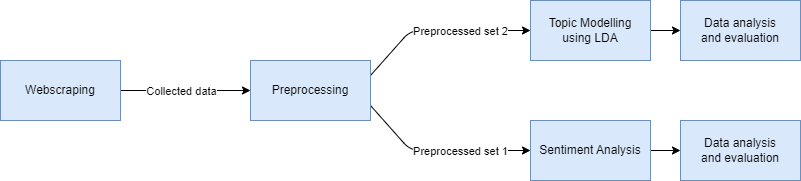
\includegraphics[width=0.8\textwidth]{resources/methodology.png}
    \caption{Summary of the methodology}
    \label{fig:methodology}
\end{figure}

The methodology can be divided into four steps: data collection via web-scraping, the preprocessing of the collected data, the processing of the preprocessed data and the analysis along with the evaluation of the analysis. The preprocessing step differs between the two analyses. The processing step is further divided into two steps: topic modeling and sentiment analysis. The following sections will discuss each step in detail.
\subsection{Data Collection}

Data collection is a crucial step in any research. When conducting a text analysis, there is more often than not a need to collect data from the internet. The difficulty of this task can vary depending on the source of the data. For example, data from social media platforms or research portals is often easier to collect than data from websites. This is because these platforms often provide APIs that allow developers to collect data. On the other hand, other websites do not always provide APIs. In such cases, researchers may have to resort to webscraping. Webscraping is a method of automatically extracting, combining and saving data from websites. The paper uses webscraping to collect data from scamalert.sg.

\subsubsection{Scamalert}

Scamalert is a website run by the National Crime Prevention Council (NCPC), which is a non-profit organization that is committed promoting public awareness and concern about crime and to propagate the concept of self-help in crime prevention.~\citep{ncpc} Scamalert contains educational sources to help people protect themselves from scams as well as provide information about acting after falling victim to a scam.

Most relevant to this paper is the section "Scam Stories". Persons who experience a crime can share their stories on the website. The stories can be sent anonymously and are published on the website. The stories are well-formatted, all containing a title, date, category, and the story itself.

Scamalert does not provide an API to access the stories. Therefore, webscraping was used to collect the data. 

\subsubsection{Webscraping}

The webscraping process was done using four libraries in Julia. Julia is a contemporary programming language that is designed for high-performance computing which is favored among data scientists. % TODO: Add citation
The four libraries in use were:

\begin{itemize}
    \item HTTP.jl: A library for making HTTP requests and handling responses 
    \item Gumbo.jl: A library for parsing HTML documents
    \item Cascadia.jl: A library for querying HTML documents using CSS selectors
    \item JSON.jl: A library for parsing JSON documents
\end{itemize}

The first step of webscraping is figuring out the structure of the website to find an efficient way of scraping the data. Fortunately, the website was well-structured. The \texttt{/stories} directory contains all the pages with stories. The stories are paginated, with each page containing data about 6 stories. The pages contained a lot of metadata about the stories, but the most important were the following: title, date, category, URL and description of the story. The story itself is not included in the page. 

This meant that the webscraping needed to be done in two steps. The first step was to collect the metadata of the stories. This was done through POST requests using HTML.jl. The requests were then parsed into JSON documents using JSON.jl then saved locally on the computer. The second step was to collect the stories themselves. This was done by iterating through the JSON documents and collecting the URLs of the stories. The URLS were then used in GET requests to collect the HTML documents of the stories. The HTML documents were then parsed using Gumbo.jl. The stories were then extracted from the HTML documents using CSS selectors provided by Cascadia.jl. The stories were then saved locally on the computer.

The data was collected on the 10th of July 2023. On the first step, a total of 590 pages were scraped, containing a total of 3536 stories. It was observed later in the process that the requests did not contain the category of the scams. This was not remedied as the category was not considered for the analysis.

The second step retrieved 3495 stories, which is 41 stories less than expected. The process of scraping was logged. The logs have shown that there were 41 errors. The errors were not caused by connectivity issues, but rather by selector issues encountered by Cascadia.jl. Upon further investigation, it was found that the cause of the errors was the HTML documents themselves. The retrieved HTML documents contained an error that is likely caused by the website host deleting the story.

After the webscraping step, a decision was made to switch to Python as the choice for a programming language. While Julia does have many data analysis libraries, it was decided that Python's ecosystem is more robust and enables more room for experimentation with the data. 

\subsubsection{Data Preprocessing}

Another important step of data analysis is the prepocessing of data. Data preprocessing can be defined as the cleaning of data and parsing it into a format that is suitable for further processing. An example of this is the removal of non-english stories, since the analysis aims to only consider stories written in english. There were a total of 5 non-english stories. The stories were removed from the dataset.

Since the aim is to do a text analysis, it is necessary to use natural language processing (NLP). NLP combines aritificial intelligence and linguistics to enable "understanding" of content. NLP is critical for topic models, as it is used to bring the text into a format that is suitable for topic modeling. Preprocessing also increases the accuracy of both topic models and sentiment analyses.~\cite{haddi2013role}\cite{chauhan2021topic}

\subsubsection*{Preprocessing for Topic Modeling}

The preprocessing step for the topic model is illustrated in the following figure (figure 2):

\begin{figure}[h]
    \centering
    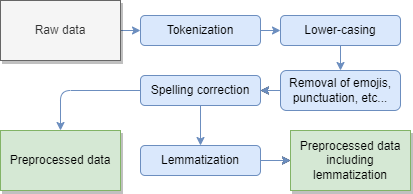
\includegraphics[width=0.6\textwidth]{resources/preprocessing_topic_modeling.png}
    \caption{Data preprocessing for topic modeling. Two datasets are produced, one is with lemmatization and one is without.}
    \label{fig:preprocessing_topic_modeling}
\end{figure}

The preprocessing was done using the Natural Language Toolkit (NLTK) library. Using NLTK, the text was tokenized, brought to lower-case, stripped off of punctuation, numbers, stopwords and emojis. Then the data was split into two sets: a set with lemmatizing and a set without lemmatizing. Lemmatizing is the process of reducing words to their root form. For instance, the word "writing" is reduced to "write". While lemmatization is a common preprocessing step, the decision to split the data was made on the basis of the claim that lemmatization correlates negatively with human interprability of english topic models.~\cite{schofield2016comparing} An example of a sentence that is preprocessed is illustrated in the table below:


\begin{table}[h]
    \centering
    \begin{tabular}{cc}
        Original & Preprocessed \\ \hline
        I was scammed by a fake website. & scam fake website \\
        \\
        Original & Preprocessed (without lemmatization) \\ \hline
        I was scammed by a fake website. & scammed fake website \\
    \end{tabular}
    \caption{Example of a preprocessed sentence. The word "scammed" was not returned to its root form in the second table.}
    \label{tab:preprocessing}
\end{table}

Additionally, the TextBlob library in Python was used to correct spelling mistakes. This does not include grammatical errors. It is not a usual practice to correct for spelling errors in topic modeling. However, since the data set consists of stories written by users, there is a high chance of spelling errors. 

\begin{figure}[h]
    \centering
    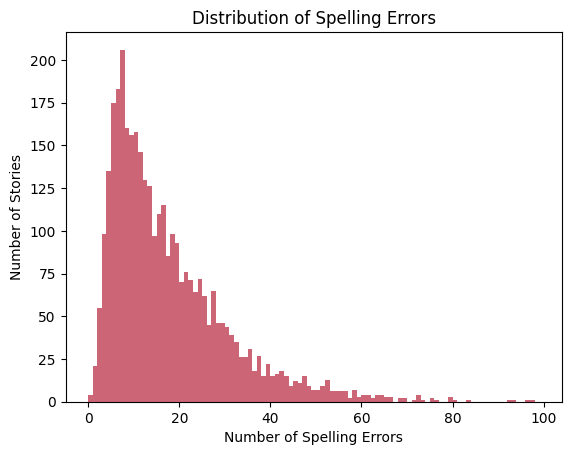
\includegraphics[width=0.8\textwidth]{resources/spelling_mistakes_distribution.png}
    \caption{Distribution of spelling errors}
    \label{fig:spelling_error_distribution}
\end{figure}


A spelling error analysis revealed that there was a total of 61070 spelling mistakes in 505672 words ($\approx 12\%$). The mean error was $\approx17$ errors per story. The median error was 13 errors per story. The conclusion was that the spelling errors were significant enough to warrant correction. The caveat is that the spellchecker library is not context-aware, it uses edit-distance algorithms to correct spelling errors. This means that it is possible to get corrections that false positives. For example, if the word "fraud" was mispelled as "faurd", it could be corrected to "found". However, it seemed that the benefits of correcting spelling errors outweighed the risks. The idea was that a false positive would appear too infrequently to have an impact on the analysis, while a true positive would contribute to the accuracy of it.

\subsubsection*{Preprocessing for Sentiment Analysis}

The preprocessing for sentiment analysis was simpler than that of topic modeling. The text was sentence-tokenized then split into two datasets, one with spelling correction and one without. Extensive preprocessing will likely remove lexical features that are important for sentiment analysis. Emojis and negations are simple examples of this. This will be elaborated further in the section about sentiment analysis.

\begin{figure}[h]
    \centering
    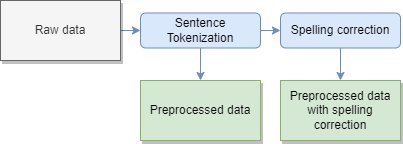
\includegraphics[width=0.6\textwidth]{resources/preprocessing_sentiment_analysis.png}
    \caption{Data preprocessing for sentiment analysis. Two datasets are produced, one is with spelling correction and one is without.}
    \label{fig:preprocessing_sentiment_analysis}
\end{figure}
\subsection{Data Analysis}

A total of 3489 stories will be analyzed in two parts: a topic model using Latent Dirichlet Allocation (LDA) and a sentiment analysis using the VADER sentiment analysis tool. The topic model will be used to identify the most common topics in the stories and the sentiment analysis will be used to identify the sentiment of the stories.

\subsection{Topic Modelling}

As mentioned in the introduction, topic modeling is a text-mining method to identify and classify data. More specifically, topic modeling is used to identify topics in a corpus of documents and classifying a distribution of words to them. A simple example would be that a sentence containing the words "politician bill government president economic growth" could be attributed to a topic "politics". We can also see that the words "economic" and "growth" could also be attributed to another topic "economy". Topic modeling extrapolates this idea to a corpus of documents and identifies the most common topics in the corpus. There are many methods to perform topic modeling, all with their own use cases, as well as advantages and disadvantages.~\cite{abdelrazek2022topic} For example, Non-negative Matrix Factorization (NMF) and BERTopic are examples of topic models that are more suited for tweets than other topic models like Latent Dirichlet Allocation (LDA).~\cite{egger2022topic} LDA seems to be frequently used to analyze abstracts of scientific papers, which are similar in length to the stories in the dataset. This was the basis for the decision to use LDA topic modeling in this project.

\subsubsection{Latent Dirichlet Allocation (LDA)}

LDA was proposed in 2003 by Blei, Ng and Jordan. It is a generative probabilistic model that assumes that each document is a mixture of topics and that each word in the document is attributable to one of the document's topics.~\cite{NIPS2001_296472c9} The most basic assumptions are the following:

\begin{itemize}
    \item There are $K$ topics in the corpus of documents that are distributed according to a Dirichlet distribution with the hyperparameter $\alpha$.
    \item Each document is a mixture of the $K$ topics.
    \item Each word in the document is attributable to one of the $K$ topics and is distributed according to a Dirichlet distribution with the hyperparameter $\beta$.
\end{itemize}

For this paper, the LDA module of python's gensim library is used.~\cite{rehurek_lrec} The gensim LDA implementation is based on Hoffman and David's implementation. The above-mentioned distributions are considered to be the prior distributions. The posterior distributions are then calculated using collapsed Gibbs sampling.

\subsubsection{Parameter Tuning}

Just like with any other machine learning model, there are parameters that play a crucial role in the accuracy of the model. These parameters are assumptions that we have to make. However, choosing the right parameters can be a complicated process.

\subsubsection*{Evaluation Metric}

Topic models should produce results that are interpretable by humans. This should be the metric that is used to evaluate the model. Obviously, it is not feasible to evaluate all models by hand. Instead, we can use metrics that are correlated with human interpretability. Examples of such metrics are the coherence score and the perplexity score. However, perplexity is not a good metric for topic models, as there are indications that it correlates negatively with human interpretability. The coherence score is a better metric, but it is not perfect either.~\cite{egger2022topic} Furthermore, there are different types of coherence scores, like the $C_v$ coherence score, the $C_{uci}$ coherence score and the $C_{npmi}$ coherence score. The $c_v$ coherence score is the most commonly used coherence score. Based on the claim that the $C_v$ score correlates highest with human ratings, it will be used in this project.~\cite{roder2015exploring} The coherence score is a value between 0 and 1, with 1 being the highest coherence score. Though high values may indicate a "too good to be true" case.  %TODO: Add source%

\subsubsection*{The Parameters}

The coherence of a produced topic model depends on the assumptions it makes. In other words, the choice of hyperparameters decides how coherent the model is, therefore it is important to choose the right parameters. The parameters to consider are listed in table \ref{tab:parameters}:

\begin{table}[h]
    \centering
    \begin{tabular}{cl}
        \hline
        Parameter & Description \\
        \hline
        $K$ & Number of topics \\
        $\alpha$ & The hyperparameter of the Dirichlet distribution of the topics\\
        $\beta$ & The hyperparameter of the Dirichlet distribution of the words  \\
          &  in each topic \\
        $min\_df$ & Minimum proportion of documents a word must appear in \\
        $max\_df$ & The maximum proportion of documents a word can appear in \\
\end{tabular}
    \caption{Parameters to consider when tuning the LDA model.}
    \label{tab:parameters}
\end{table}

As mentioned before, the LDA model has two hyperparameters $\alpha$ and $\beta$. In this project, $\alpha$ is a singular scalar value that is used for all topics. For example, if we have $K=3$ topics and $\alpha=0.1$, then the Dirichlet distribution for the topics would be $\textbf{Dir}(0.1, 0.1, 0.1)$. $\beta$ is as well a singular scalar value that is used for all words in the corpus. For example, if we have $V=1000$ words in the corpus and $\beta=0.1$, then the Dirichlet distribution for the words would be $\textbf{Dir}(0.1, 0.1, ..., 0.1)$ with $V$ values.

Due to the nature of Dirichlet distributions, low values of hyperparameters produce sparse distributions, while high values produce more uniform distributions. This means that low values of $\alpha$ assume that each document will be dominated by a few topics, while high values assume that each document will contain a mixture of more-or-less all topics. Similarly, low values of $\beta$ assume that each topic will be dominated by a few words, while high values assume that each topic will contain a mixture of more words.

\begin{figure}[h]
    \centering
    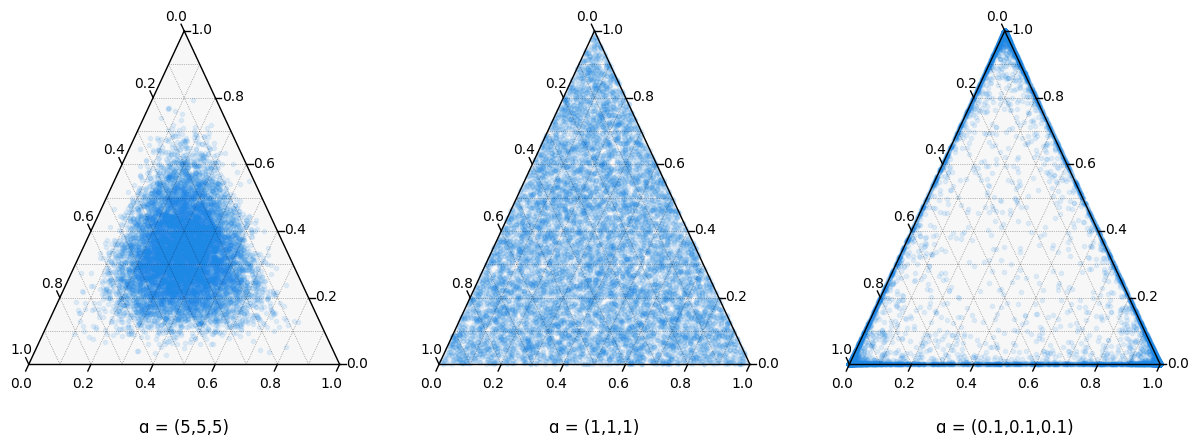
\includegraphics[width=1\textwidth]{resources/dirichlet_example.png}
    \caption{Scatter plots of 10000 samples of dirichlet distributions with different values of $\alpha$. For higher values, the distributions are more concentrated in the center. In the context of LDA, this means that each is assumed to have similar proportions of each topic for each document.}
    \label{fig:spelling_error_distribution}
\end{figure}


The number of topics $K$ is a parameter that is not related to the Dirichlet distributions. It is the number of topics that the model will try to identify.

The parameters $min\_df$ and $max\_df$ are used to filter out words that are too common or too rare, as such words may hurt the coherence of the model. For example, if a word occurs very frequently in a small corpus, it could be attributed to a topic that it is not coherent to. Likewise for words that may rarely occur in a large corpus. The values of these parameters completely depends on the corpus of documents.

\subsubsection*{Tuning the Parameters}

The parameters are not independant of each other. Every combination of the parameters yields a different coherence score, and the aim is to maximize this score. Two common approaches to parameter tuning are grid search and randomized search. 

Grid search is a brute force approach that tries every combination of parameters. The user specifies a range of values for each parameter and the algorithm tries every combination of these values. At the end, the combination of parameters that yields the highest coherence score is chosen. There are some problems with this approach. Firstly, it is computationally expensive. Producing an LDA model can take a long time. Calculating coherence scores for each set of parameters means that a module must be produced using the parameters, and then the coherence score must be calculated. Depending on the parameter values, this can take a long time. For example, the first grid search that was performed for this project used a relatively conservative range of values for the parameters (around 7 values for each parameter), which resulted in 38000 models being produced, this took over 24 hours to complete. This means that the number of parameter values need to be limited in order to make the grid search feasible, which leads us to the second issue with this approach, which is that the best parameters may not be in the range of values that were specified. This means that the best parameters may not be found. Additionally, the grid search could cause overfitting, as the parameters are chosen based on the coherence score, which is calculated using the same data that the model was trained on.

The more feasible alternative to grid search is the randomized search. This approach is similar to grid search, but instead of trying every combination of parameters, it tries a random sample of the combinations for a set number of iterations. This allows for a larger range of values to be specified for the parameters, while keeping the task computationally feasible. In fact, the randomized search produced a higher range of coherence scores than the grid search, while taking less time to complete. 5000 models were evaluated in less than 4 hours, yielding a highest coherence score of over 0.38, while the grid search yielded the highest coherence score of 0.37. While this is not a significant difference, it makes evaluation a much cheaper and accessible task. Of course, the randomized search is not guaranteed to find the best parameters, but it is a good compromise between the grid search and the manual tuning of parameters. Interestingly, Bengstra and Bengio (2012) say that randomized search is theoretically and emperically more efficient than grid search, while obtaining results that are just as good or sometimes better than grid search.~\cite{bergstra2012random}
\subsection{Sentiment Analysis}

Many texts are written purely to convey information without intentions of containing any sentiment. Defining sentiment can be a tricky task, but as many other researchers do, this paper uses the loose definition of sentiment as "negative or positive opinion".~\cite{mejova2009sentiment} This definition may be viewed as too simplistic or reductionist, but it has its benefits.

Research papers and textbooks tend to be written in a neutral tone, evasive of any sentiment. On the other hand, texts like novels, poems, songs and social media posts are often written with the intention of conveying sentiment. Answering the question: "What do people feel about a certain subject?" is valuable for companies and organizations. By understanding public opinion, companies and organizations can gain insights, improve their decision-making or use it as a form of feedback to improve their products and services.~\cite{mejova2009sentiment}

Given the data that has been collected for this paper, it is interesting to ask: "What are the sentiments of stories told by cybercrime victims?" Intuitively, one would expect pre-dominantly negative sentiments, but if there is positive sentiment, it would be interesting to know why. Moreover, it is interesting to know the intensity of the sentiment. Are the stories very negatively told? Are they slightly negative? And so on.

\subsubsection*{Method}

Just as with topic modeling, it is of course possible but time-consuming to manually read texts and categorize it into sentiment. Sentiment analysis is a way of automating this process. Sentiment analysis is a natural language processing technique that extracts sentiments from texts. Since sentiment is considered to be an opinion, it is a subjective measure, making it difficult to extract. An advantage of the simplistic definition given above is that it is of categorical nature, which makes it a task for supervised machine learning. Given a data set of texts and their sentiment, a machine learning model can be trained to predict the sentiment of a text.

However, as expected, Scam Alert does not provide sentiment labels for the stories told by their users, making the machine learning based approach out of scope for this paper. Beside the labeling issue, machine learning approaches have other problems like computing costs and requiring extensive amounts of data.~\cite{hutto2014vader} Alternatively, a lexicon based approach can be used. Lexicons don't typically contain information about sentiment, but some lexicons have been developed that do, so-called sentiment lexicons. A sentiment lexicon is a list of words that are annotated with a sentiment score.~\cite{bonta2019comprehensive} For example, Valence Aware Dictionary and sEntiment Reasoner (VADER) is a sentiment lexicon, which also describes sentiment intensity, that contains over 7,500 words and emoticons that are annotated with a sentiment compound score between -4 and 4, -4 being most negative, 0 being neutral and 4 being most positive.~\cite{hutto2014vader} The NLTK library contains a sentiment analysis implementation that uses the VADER lexicon, which is used in this paper. The compound score is normalized to be a value between -1 and 1 in the NLTK implementation. The NLTK implementation also provides the proprotion of negative, neutral and positive sentiment in a text.

\begin{table}
    \centering
    \resizebox{\textwidth}{!}{
        \begin{tabular}{lllll}
            \hline
            \textbf{Sentence} & \textbf{Negative} & \textbf{Neutral} & \textbf{Positivity} & \textbf{Compound} \\ \hline
            'It was a giant disaster.' & 0.672 & 0.328 & 0.0 & -0.6249 \\
            'I felt supported.' & 0.0 & 0.303 &  0.697 & 0.3182\\ 
            'The caller introduced himself.' & 0.0 & 1 &  0 & 0\\ \hline
        \end{tabular}
        }
    \caption{Examples of sentiment analysis results on different unprocessed texts.}
    \label{tab:sentiment_analysis_example}
\end{table}

There are also new modern approaches to sentiment analysis that combine supervised learning with lexicon based approaches that seem to generally present better results than solely machine learning based approaches.~\cite{ahmad2017hybrid} Since lexicon-based approaches are rule-based, there will be cases where sentiment extraction won't be very accurate. The hybrid approach mends this problem by compensating for the shortcomings of the lexicon-based approach with the machine learning based approach. However, the hybrid approach was deemed out of scope for this paper.

\subsubsection*{The VADER Lexicon}

The VADER lexicon is a simple rule-based model for sentiment analysis. It is a gold-standard lexicon that was empirically validated by independent human raters. It expands on well-established lexicons that existed before it, namely General Inquirer (GI), Linguistic Inquiry and Word Count (LIWC) and the Affective Norms for English Words (ANEW). Moreover, it recognizes additional lexical features like emoticons, acronyms and slang, which are commonly used in social media.~\cite{hutto2014vader}

VADER is tuned to the process of word-sense disambiguation, which is the process of determining the meaning of a word in a sentence depending on the context. An example by the authors of the VADER lexicon is the word "catch", which can be used in a negative sense, like "At first glance the contract looks good, but there's a catch". But the word "catch" can also be neutrally. The sentence "The fisherman plans to sell his catch at the market" illustrates this.~\cite{hutto2014vader}

Being "rule-based" refers to the fact that the VADER lexicon uses a set of rules to determine the sentiment of a text. The rules are based on the following heuristics:

\begin{enumerate}
    \item Punctuation, capitalization, degree modifiers and conjunctions increase the magnitude of the sentiment score.
    \item Adverbs increase the magnitude of the sentiment score.
    \item Negations reverse the polarity of the sentiment score.
    \item Emojis and emoticons are scored positively.
    \item Words in ALL CAPS are scored more strongly.
\end{enumerate}

This makes the VADER lexicon a good choice for social media texts, since they often contain the above-mentioned features, which affect the perceived sentiment of a text. This is an advantage over bag-of-words approaches, which don't consider the order of words.

\begin{table}
    \centering
    \begin{tabular}{lc}
        \hline
        \textbf{Sentence} & \textbf{Compound Score} \\ \hline
        'I didn't feel good about it.' & -0.3412  \\
        'I felt awful about it.' & -0.4588 \\ 
        'I felt AWFUL about it.' & -0.5766 \\ 
        'i felt AWFUL about it!!!' & -0.6817 \\ \hline
    \end{tabular}
    \caption{The sentiment compound score of a text is affected by punctuation, capitalization and degree modifiers.}
    \label{tab:sentiment_analysis_heuristics_effects}
\end{table}


The VADER lexicon performs in most cases better than 11 other well-established lexicons. In a case of analyzing 4,200 tweets, it even performed better than human raters.~\cite{hutto2014vader} It was also externally validated to perform better than alternatives.~\cite{al2020evaluating}\cite{min2020comparative}

Being an empirically validated lexicon that is suitable for interpreting social media texts, the VADER lexicon was chosen for this paper. The stories told by the victims contain many of the features that the VADER lexicon is tuned to, like emoticons and emphasis through capitalization and punctuation.


\subsection{Topic Model}

5000 iterations of randomized search were performed to find the optimal parameters for the topic model. The highest score was $0.3867$ and the lowest was $0.1975$. 6 of the 5000 models had a coherence score higher than $0.38$.

Two models are presented for good measure. The highest coherence score was $0.3867$, followed by a score of $0.3842$. The parameters of the corresponding topic models are listed in table 5 as well as other data. An interactive visualization of both models using pyLDAvis is available in the appendix.

Figure 6 shows a visualization of the topics of model 1 and the distribution of the top 20 most common words in them.

\begin{table}[!h]
    \centering
    \begin{tabular}[\textwidth]{lcccccc}
        \hline
        \textbf{Model}  & No. Topics & $\alpha$ & $\beta$ & min\_df & max\_df & $C_v$ \\ \hline
        Model 1 & 2 & 0.05 & 0.02 & 0.07 & 0.30 & 0.3867 \\
        Model 2 & 6 & 0.07 & 0.05 & 0.02 & 0.20 & 0.3842 \\ \hline
    \end{tabular}
    \caption{Parameters of the topic models.}
\end{table}

\begin{figure}[H]
    \centering
    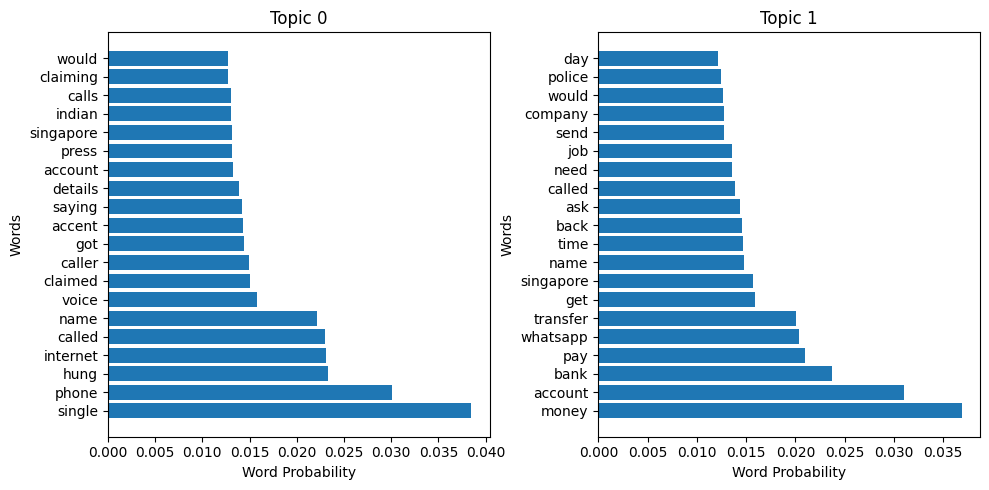
\includegraphics[width=\textwidth]{resources/model_n_2.png}
    \caption{Visualization of the topics in model 1.}
    \label{fig:topic_model_1}
\end{figure}

Topic 0 was present in 55.7\% of all documents, while topic 1 was present in 60.2\%. Using gensim's implementation of the Hellinger Distance, a metric to measure the similarity between two probability distributions, the distance between the two topics was $0.45$.

\begin{figure}[H]
    \centering
    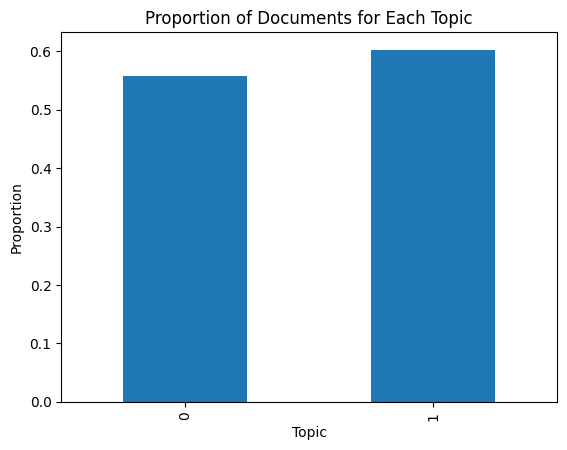
\includegraphics[width=0.5\textwidth]{resources/proportion_n_2.png}
    \caption{Proportion of model 1 topics in the corpus.}
    \label{fig:proportion_n_2}
\end{figure}

Model 2, which contains 6 topics, is visualized similairily below in figures 8 and 9. The most prominent topic in the corpus is topic 0, which is present in 35.7\% of all documents, followed by topic 5 at 32.8\%, topic 2 at 32.1\%, topic 4 at 31.3\%, topic 3 at 25.2\% and topic 1 at 23.0\%.

\begin{figure}[H]
    \centering
    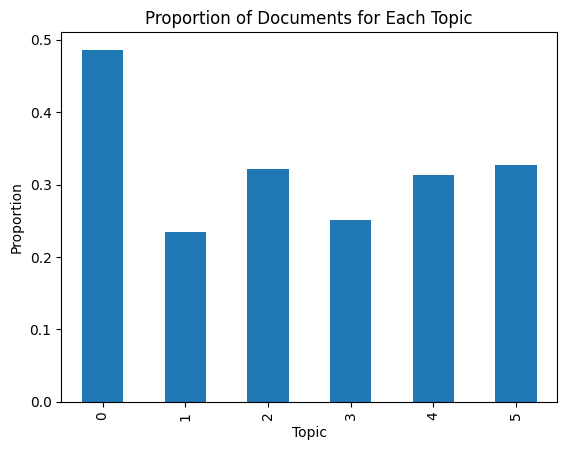
\includegraphics[width=0.5\textwidth]{resources/proportion_n_6.png}
    \caption{Proportion of model 2 topics in the corpus.}
    \label{fig:proportion_n_6}
\end{figure}

Since the number of topics is higher than 2, the Hellinger Distance is presented as a matrix that shows the distance between each pair of topics. The matrix is shown in table 6.

\begin{table}[H]
    \centering
    \resizebox{\textwidth}{!}{
      \begin{tabular}{|*{7}{>{\centering\arraybackslash}m{2.9cm}|}}
            \hline
            Topic & 0 & 1 & 2 & 3 & 4 & 5 \\
            \hline
            0 & 0.000 & 0.503 & 0.498 & 0.463 & 0.533 & 0.439 \\
            \hline
            1 & 0.503 & 0.000 & 0.430 & 0.448 & 0.421 & 0.446 \\
            \hline
            2 & 0.498 & 0.430 & 0.000 & 0.405 & 0.386 & 0.388 \\
            \hline
            3 & 0.463 & 0.448 & 0.405 & 0.000 & 0.425 & 0.429 \\
            \hline
            4 & 0.533 & 0.421 & 0.386 & 0.425 & 0.000 & 0.437 \\
            \hline
            5 & 0.439 & 0.446 & 0.388 & 0.429 & 0.437 & 0.000 \\
            \hline
        \end{tabular}
      }
    \caption{Hellinger Distance matrix of model 2.}
    \label{tab:hellinger_distance_matrix}
  \end{table}

\begin{figure}[H]
    \centering
    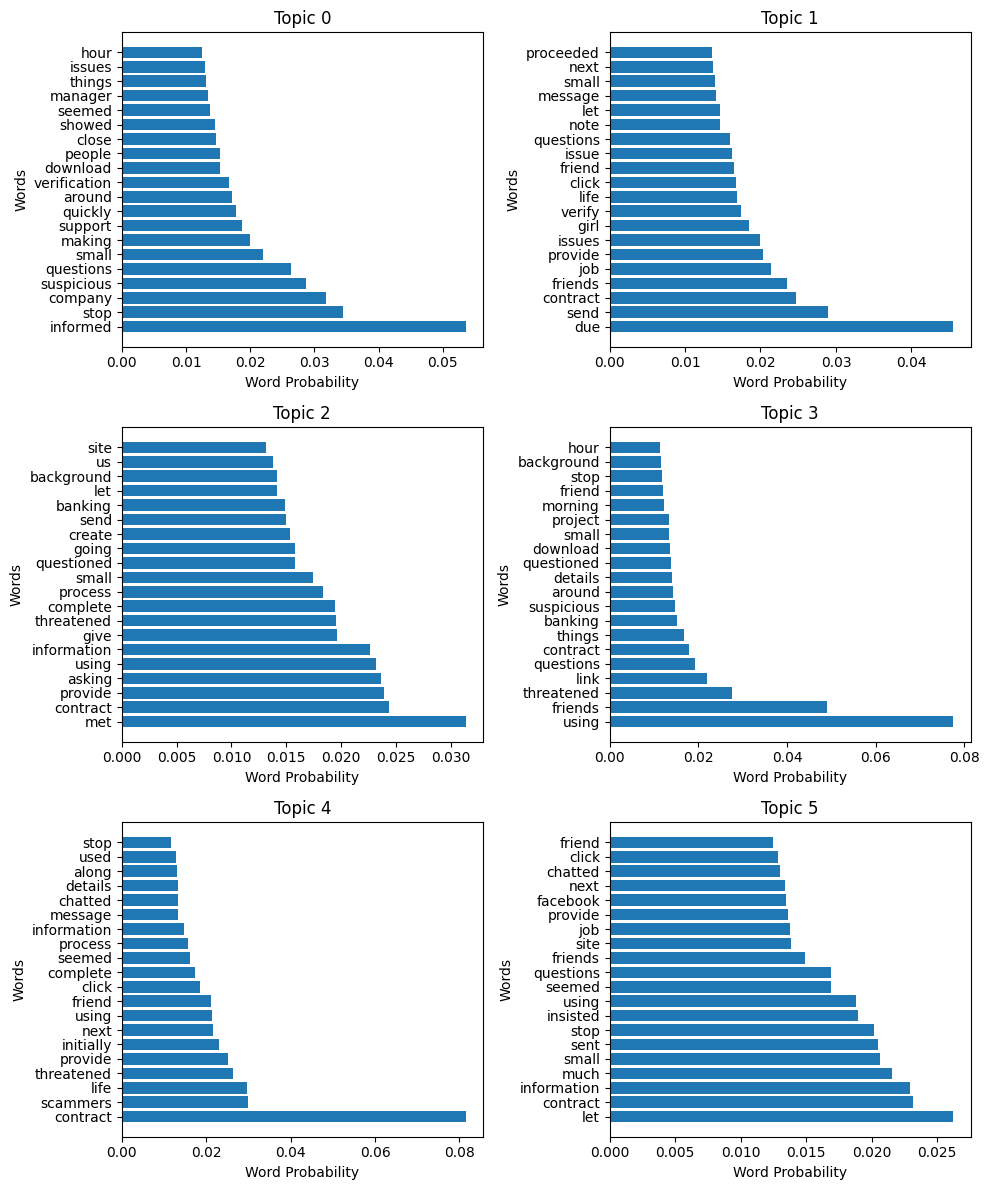
\includegraphics[width=\textwidth]{resources/model_n_6.png}
    \caption{Visualization of the topics in model 2.}
    \label{fig:topic_model_2}
\end{figure}
\subsection{Sentiment Analysis}
\label{sec:sentiment_analysis}

The sentiment analysis examines 29,096 sentences extracted from all the stores. For each sentence, a compound score was calculated. Additionally, the proportion of negativity, neutrality and positivity of each sentence was also calculated.

Neutral sentiment sentences have a compound score of 0. Negative compound scores are considered to be a negative sentiment, and values higher than 0 are considered to be positive. Table \ref{tab:sentiment_proportion} shows the proportion of each sentiment in the data sets.

\begin{table}
    \centering
    \begin{tabular}{llll}
        \hline
        Data set & Positive & Neutral & Negative \\ \hline
        With spell-correction & 0.31 & 0.41 & 0.23 \\
        Without spell-correction & 0.31 & 0.42 & 0.27 \\
        \hline
    \end{tabular}
    \caption{Proportion of sentiments in the data sets. Values are rounded to two decimal places.}
    \label{tab:sentiment_proportion}
\end{table}

The mean compound score of the data set with spell-correct is 0.00 with a standard deviation of 0.35, while that of the set without spell-correct is also 0.00 with a standard deviation of 0.35. Figure \ref{fig:sentiment_distribution} shows the distribution of the compound scores in both data sets and table \ref{tab:sentiment_analysis} shows a summary of the distribution that includes the maximum and minimum values.

\begin{figure}[H]
    \centering
    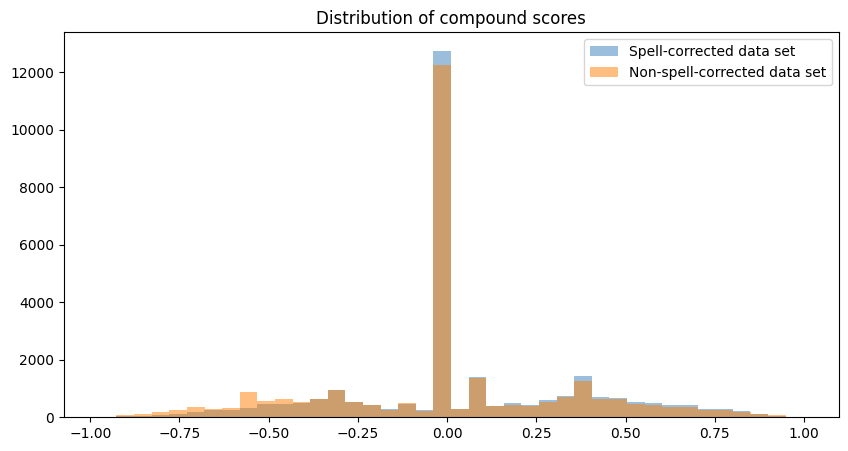
\includegraphics[width=\textwidth]{resources/compound_scores.png}
    \caption{Distribution of the compound scores in the data sets.}
    \label{fig:sentiment_distribution}
\end{figure}

\begin{table}
    \centering
    \resizebox*{\textwidth}{!}{
        \begin{tabular}{lcccc}
            \hline
            Data set & Mean & Standard deviation & Minimum & Maximum \\ \hline
            With spell-correction & 0.00 & 0.35 & -0.98 & 1.00 \\
            Without spell-correction & 0.00 & 0.35 & -0.98 & 1.00 \\
            \hline
        \end{tabular}
    }
    \caption{Description of the sentiment analyses distributions.}
    \label{tab:sentiment_analysis}
\end{table}

The distribution of the negativity proportions in sentences is shown in figure \ref{fig:negativity_distribution}.

\begin{figure}[H]
    \centering
    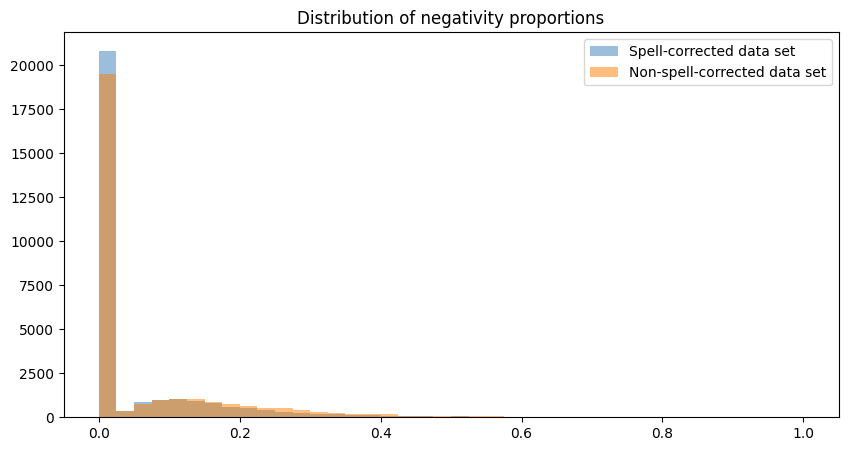
\includegraphics[width=\textwidth]{resources/negativity_distributions.png}
    \caption{Distribution of the negativity proportions in the data sets.}
    \label{fig:negativity_distribution}
\end{figure}

The non-spell-corrected data set contains 9,619 with negativity proportions larger than 0, while the spell-corrected data set contains 9,706. This is a difference of 87 sentences.

The positivity proportions are presented in the same fashion in figure \ref{fig:positivity_distribution}.

The non-spell-corrected data set contains 11,443 sentences with positivity proportions larger than 0, while the spell-corrected data set contains 11,579. The spell-corrected data set contains 136 more sentences with positive proportions.

The non-spell-corrected data set has 1,160 more positive sentences than negative sentences, meaning sentences with compound scores over 0, while the spell-corrected data set has 1,170 more positive sentences than negative sentences.


\begin{figure}[H]
    \centering
    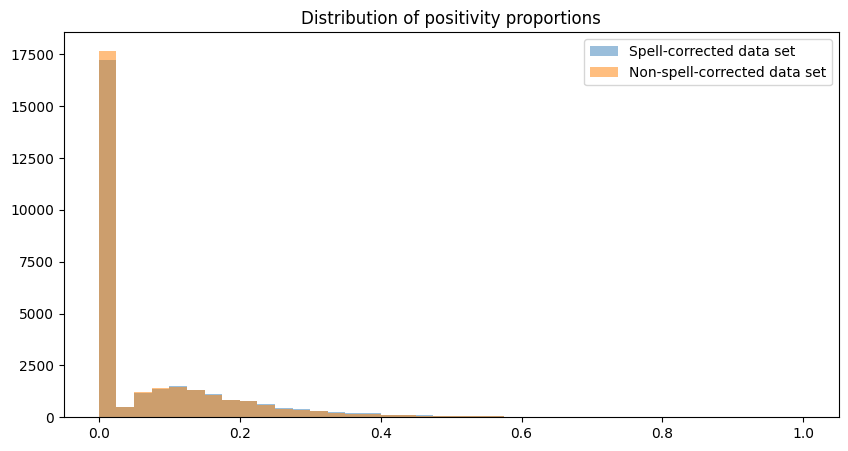
\includegraphics[width=1\textwidth]{resources/positivity_distributions.png}
    \caption{Distribution of the positivity proportions in the data sets.}
    \label{fig:positivity_distribution}
\end{figure}

The distributions of all proportions are visually shown in figure \ref{fig:proportions}.

\begin{figure}[H]
    \centering
    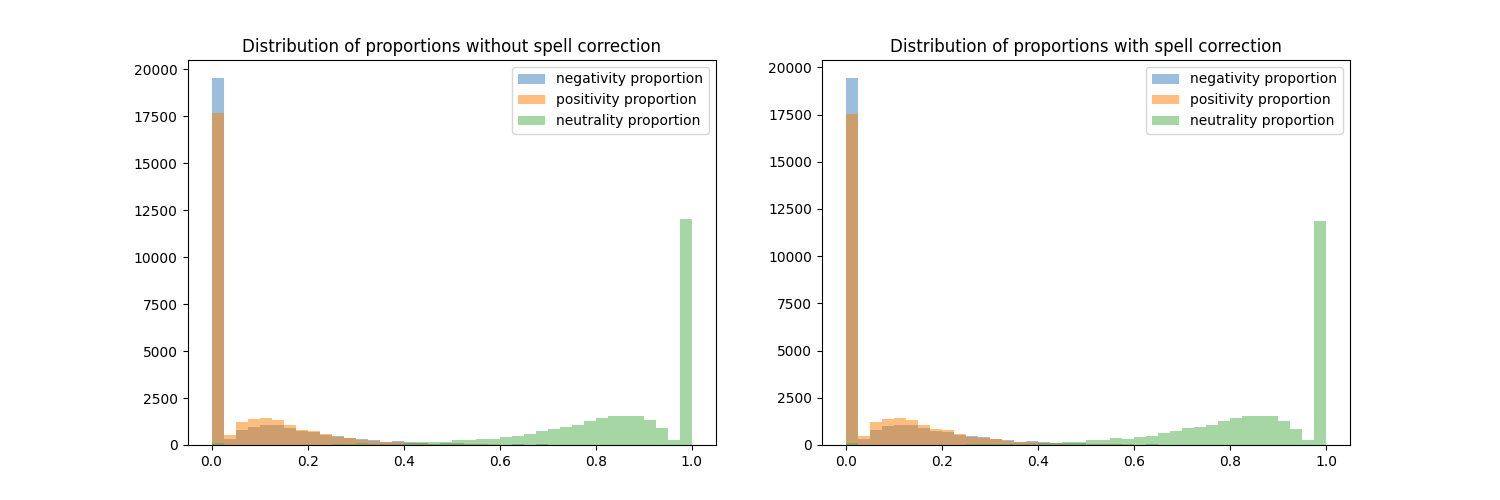
\includegraphics[width=1\textwidth]{resources/proportions.png}
    \caption{Distribution of the positivity proportions in the data sets.}
    \label{fig:proportions}
\end{figure}
\section{Discussion}

\subsection*{Key Findings}

The analyses produced unexpected results that do not adequately answer the research questions formulated in the introduction. The topic models are not very informative and can be interpreted in many ways, which is not what a topic model should produce.

The sentiment analysis results are also quite surprising. One would expect encounters with cybercrime to provoke negative emotions, but the results show that the majority of the sentences are neutral. What is more surprising is that positive sentiments are more common than negative ones. Furthermore, spell correction during preprocessing did not significantly affect the general sentiment.

\subsection{Topic Models}

The two presented topic models both had coherence scores of over 0.38. It is not possible to state whether this is an acceptable score or not, as the metric only correlates to human interpretability. However, the models produced did not seem to contain interpretable topics. Most topics contained a mix of words that does not construct a context.

One topic that could be considered as interpretable was topic 1 of model 1. The top 5 words were "money", "account", "bank", "pay", "whatsapp", "transfer", which seems to be related to monetary transactions. However, the top 15 words included words like "singapore", "time", "ask", which are not necessarily related to monetary transactions. The rest of the topics were even less interpretable.

\begin{figure}[H]
    \centering
    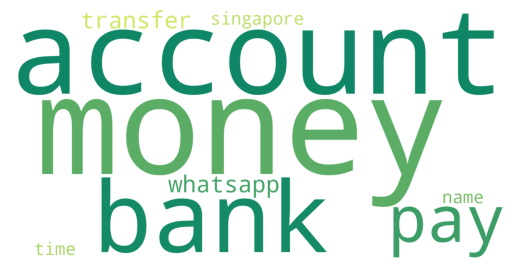
\includegraphics[width=0.5\textwidth]{resources/word_cloud1.png}
    \caption{Word clouds of the top 15 words of the topics of model 1.}
    \label{fig:wordclouds}
\end{figure}

Interestingly, model 2 did not produce topics that could be interpreted as related to monetary matters, unlike model 1. This could be an indicator the parameters chosen are not a good fit, since financial damages are very likely to happen in cybercrime cases.

There was no answer to the question of how victims cope with cybercrime. Some words like "friends" or "police" were present in some topics, which are ways that victims might turn to as coping mechanism, but the topics were not interpretable enough to draw any conclusions.

The Hellinger distance between the topics of model 1 was 0.45 indicating that the topics are not very similar, but also not very different. Model 2 averaged a distance of 0.44, which is very similar to model 1. This is somewhat surprising, as the topics of model 2 seem to be more similar to each other. For example, the words "contract", "information" and "friends" (or "friend") are present in at least half of all topics. On the other hand, the topics of model seem to be more diverse when comparing the top words. Of the top 20 words in model 1, only 4 words were present in both topics.

Overall, the topic models are deemed to be not very informative and do not contribute to answering the research questions. There are a few possible reasons for this relating to the process of LDA and the data it was conducted on.

\subsubsection*{The Data}

Machine learning processes depend largely on the data they train on. As mentioned before, noisy data produces noisy results. However, the data used in this project were preprocessed in a commonly practiced way and avoided a common preprocessing step that hurts interpretability, namely lemmatization.~\cite{schofield2016comparing} Though spelling correction is not a common practice, it likely did not increase noise, as false positives most likely appeared too infrequently to have an impact on the analysis. For instance, with a minimal $min\_df$ value of 0.02, a word needs to appear in at least 70 stories to be considered. It is very likely that a false positive would appear in 70 separate stories and be frequent enough to be considered a topic word. Though the research community could benefit from a more thorough scrutinization of the effects of spelling correction on topic models rather than relying on heuristics similar to the one used in this paper.

What shouldn't be ruled out is the size of the data as well as its linguistic structure. It is not clear how much data is needed to produce a good topic model. This will depend on a couple of factors, like the length of the documents in the corpus, and what writing style is used. Stories told by victims on Scamalert have a similar length to academic paper abstracts, but differ in that they are written informally. The impact of this on LDA is not very clear, and it is possible that the dataset is not large enough to produce good results.

\subsubsection*{Coherence as a Metric}

Goodhart's law describes that when a measure becomes a target, it ceases to become a good measure. It has its origins in economics and later found applications in social sciences.~\cite{strathern1997improving}\cite{goodhart2015goodhart} Having a target measure provides incentive to maximize it, which can lead to unintended consequences. Hoyle et al. (2021) ask whether this is also applicable to coherence score as a measure.~\cite{hoyle2021automated}

While the coherence score is a widely used measure to evaluate topic models, it is by no means a gold-standard measure. It correlates with human interpretation but one cannot say whether it accurately describes it. Hoyle et al. (2021) are of the mind that the state of topic modeling today is overdue for serious reconsideration and intend to explore better automated metrics.~\cite{hoyle2021automated}

While some $K_0$ number of topics may have a high coherence score, a different number of topics $K_1$ could also have a similar coherence score but with a different set of parameters. Though both models yield high coherence scores, it cannot be true that the corpus has both $K_0$ and $K_1$ topics. This problem arises from the metric that is used to evaluate the model. This is a problem that is inherent to unsupervised machine learning models.


\subsubsection*{LDA}

It is possible that LDA is not a suitable model for this dataset. There are other alternatives to LDA that might be a better fit for this dataset and produce more interpretable results.

Being a machine learning process, topic modeling in general could also produce latent topics that are perhaps present in the data, but not interpretable by humans. This is a common problem in machine learning that is known as the "black box" problem that is being addressed by the research community, since it causes problems in high-stakes applications like healthcare, criminal justice and other domains. Rudin proposes a solution to this problem by using inherently interpretable models instead of black box models. This is a promising approach that could be applied to topic modeling as well.~\cite{rudin2019stop}

LDA is also a bag-of-words (BOW) model, so it does not account for the order of words in a document. This means that the model is not able to capture the context of words.

Another limitation is that LDA cannot capture correlations between topics. For example, if a corpus contains the topics "politics" and "tax", it is likely that there will be documents that contain both topics. However, Dirichlet distributions cannot capture this correlation.
\subsection{Sentiment Analysis}

The sentiment analysis delivered surprising results. Crime is a negative experience for its victim and one would intuitively expect victims to exhibit negative emotions when talking about their experience. However, the results indicate that the sentiment is quite neutral. But what is more counter-intuitive is that positive sentiments seem to be more common than negative ones.

\subsubsection*{False Interpretations}

Perhaps the biggest factor that affects the quality of the sentiment analysis is how the VADER lexicon interprets the data. Many sentences were not meant to contain positive nor negative sentiment, but were interpreted as such. For example, the sentence "I accepted a friend request on Facebook because we had a common friend." was interpreted as very positive with a compound score of 0.82, where it is meant to be neutral. This is likely because the word "friend" was present twice in the sentence.

The sentence "When the time came, they resorted to emotional blackmail and questioned my integrity to manipulate me into assisting them." was interpreted as quite positive too, with a compound score of 0.42. This is a confusing result, given that the words "blackmail" and "manipulate" are present in the sentence. It seems that the word "assist" was favored by the rules of the VADER lexicon and labeled the sentence as positive.

While it's not easy to count the amount of false interpretations, an inspection of the data showed that such interpretations were not so uncommon. 

\subsubsection*{The Effect of Spell Correction}

When glancing at the results presented in section \ref{sec:sentiment_analysis}, it looks like spell-correction did not significantly affect the sentiment of the data. A visual inspection of figure \ref{fig:sentiment_distribution} doesn't reveal any large notable changes in the distribution and the mean compound score differs by an insignificant fraction. A t-test reveals that the difference is statistically insignificant for all measures of the analysis, delivering (p $>$ 0.2) for the sentiment proportions and (p $>$ 0.9) for the compound score.

Upon manually inspecting 50 randomly sampled, corrected sentences, surprisingly no false positives were found. 50 sentences is not a large enough sample to make any conclusions, but it is a good indication that spell correction did not introduce many false positives.

\subsubsection*{Data Origin}

The data set contains originates from Singapore. It is possible that the cultural background of the victims affects the way they describe their experiences. Additionally, the website encourages users to share stories of their experience with crime, but users might be inclined to keep a neutral tone when sharing their stories. Scamalert looks to warn and educate people about scams, so it is possible that it's an environment that encourages neutral language. Users share also share their stories anonymously and this likely affects the way they describe their experience.

\subsubsection*{VADER Limitations}

The lexicon-based approach is not without its shortcomings: 

%% enumerate
\begin{enumerate}
    \item \textbf{Limited coverage:} The VADER lexicon is limited in its coverage. It does not contain all possible words, and it is not guaranteed to cover all possible words. This is especially true for new and emerging slang as well as domain-specific language.
    \item \textbf{Limited word-sense disambiguation:} The VADER lexicon does not perform word-sense disambiguation. For example, the word "sick" can be used to describe a disease or to describe something that is cool. The lexicon does not distinguish between the two meanings, and is up to the context to determine the meaning of the word. This is a difficult task for a machine to perform.
    \item \textbf{Sarcasm and irony:} Sarcasm and irony are very difficult to detect and are not addressed by the VADER lexicon.
\end{enumerate}

Perhaps these are limitations that can be alleviated with the machine-learning or the hybrid approach to sentiment analysis.

\subsection{Future Work}

Topic modeling and sentiment analysis are an exciting new approach to text synthesis. While the thesis has shown that no clear information was extracted from the data, there are many methods to deliver different or better results.

LDA is considered to be a state-of-the-art model for topic modeling. But it comes with its own limitations that can perhaps cause to be harmful for data sets such as the one used in this project. Applying other models such as NMF could be an alternative that produces more meaningful results.

The project used a simple lexicon-based approach to sentiment analysis, which as discussed, has its fair share of shortcomings. A new exciting approach to sentiment analysis is a combination of using topic modeling to extract topics by sentiment, so-called joint sentiment/topic models.~\cite{lin2009joint} This could be a more suitable alternative to investigate how victims feel by topic and might deliver far more meaningful results. It might be possible to extract topics linked to high negative sentiment and link them to certain feelings, such as shame or fear.

\subsubsection*{Further Research on Coping Mechanisms}

It has been shown that there is a lack of research on the psychological impact of cybercrime, let alone the coping mechanisms that victims use to recover from their experience. The research community and victims alike could benefit from more insights into the coping mechanisms that victims use to recover from their experience. Reproducing the research results, for example those of Jansen and Leukfeldt (2018) or Button et al. (2009), could be a valuable contribution~\cite{jansen2018coping}\cite{button2009better} and as conducting surveys.

\subsubsection*{Data Scarcity}

Data is very scarce in this field and there need to be more efforts towards data collection and organization. The more data there is, the more research can be done. Machine-learning based sentiment analysis could be a valuable tool to analyze the data and extract meaningful information, but this was not possible due to the lack of data, as well as labels for the data. A framework for cultivating data can increase the amount of research in the field of cybercrime victimization.


\subsubsection*{A Social Platform for Supporting Cybercrime Victims}

The context of Scamalert could be a major factor to skewing the data towards neutral sentiment. Users seem to be inclined to report their encounter rather than share their experience as a whole. A platform that is more oriented on supporting victims and helping them recover from their experience could be a better source of data. Creating an environment for victims to share and support each other could provide a valuable service to the victims of cybercrime. Jansen and Leukfeldt's research indicates that the support of others is an effective coping mechanism for victims of cybercrime.~\cite{jansen2018coping} Button et al. (2009) support this finding with their research stating that 83\% of victims feel that a sympathetic response is 'very important' (n=745).

Such a platform could also be used to improve the data ecosystem on this subject. Victims could be prompted to label their stories with the feelings they experienced, which could be used to train a sentiment analysis model. A built-in API could be used to extract the data and make it available for research purposes.
\subsection{Conclusion}

The thesis used state-of-the-art methods to analyse stories told by cybercrime victims but revealed no useful insights about the topics that victims speak about. This may support the claim that coherence is not an appropriate measure for topic models, but could also indicate that the data itself is not suitable for LDA.

Victims tended to neutrally speak about their experiences, rather than adding much sentiment to their stories. The findings are by no means conclusive and further research is crucial for further understanding the matter of cybercrime victimization.



%===========================================================
% References
%===========================================================
\bibliographystyle{plain}
\bibliography{bibliography.bib}
%===========================================================
% Appendix
%===========================================================
\section*{Appendix}

All the code used in this paper is located on a remote GitHub repository. The repository can be found at:

% list of items

\begin{itemize}
    \item \url{https://github.com/MundherAl/BachelorThesis}
\end{itemize}

A rendered view of the interactive LDA visualizations using pyLDAvis are in the following links:

\begin{itemize}
    \item LDA Model 1 \url{https://htmlpreview.github.io/?https://github.com/MundherAl/BachelorThesis/blob/main/lda_visualizations/lda_1.html}
    \item LDA Model 2 \url{https://htmlpreview.github.io/?https://github.com/MundherAl/BachelorThesis/blob/main/lda_visualizations/lda_2.html}
\end{itemize}


\pagebreak\noindent
\textbf{\LARGE Declaration}
\addcontentsline{toc}{section}{Declaration}

\bigskip\bigskip
\noindent 
I hereby confirm that I have independently written my 
bachelor's thesis and have not used any sources or aids 
other than those specified.
\bigskip
\noindent
% Date of Declaration

\bigskip\bigskip\bigskip
\noindent
% Automatic date
D\"usseldorf, \today \\
(Mundher Al-Ahmadi)


\end{document}